Neutrinos unterliegen lediglich der schwachen Wechselwirkung, womit sich sehr kleine
Wirkungsquerschnitte ergeben, beispielsweise

\[\sigma_\text{total}(\nu,\,200\,\text{GeV}) = 1{,}6\cdot10^{-36}\text{cm}^2 = 1{,}6\,\text{pb} \]

Zum Nachweis werden also sehr große Detektoren benötigt. Es finden folgende Prozesse statt:

\[ \nu_l + n \longrightarrow l^- + p \]
\[ \bar{\nu}_l + p \longrightarrow l^+ + n \]

mit $l=e,\mu,\tau$. Für den Nachweis in Kollisionsexperimenten konstruiert man einen hermetischen
Detektor: 

\begin{figure}[H]
		\centering
		\includesvg[svgpath=bilder/1-345/]{neutrino}
\end{figure}


Man kann die Energie/Impuls-Summe vor und nach der Kollision aufstellen:

\[\sum_\text{vorher} \vec{E}_\text{i} = \sum_\text{nachher} \vec{E}_\text{i}^\text{ gemessen}
+\textcolor{red}{\vec{E}_\nu}\]

mit der Annahme, dass der fehlende Energie-Impuls-Vektor vom Neutrino stammt. Ein direkter Nachweis
ist auch möglich mit extrem massiven Targets und hohen Neutrinoflüssen.

\begin{figure}[H]
	\centering
	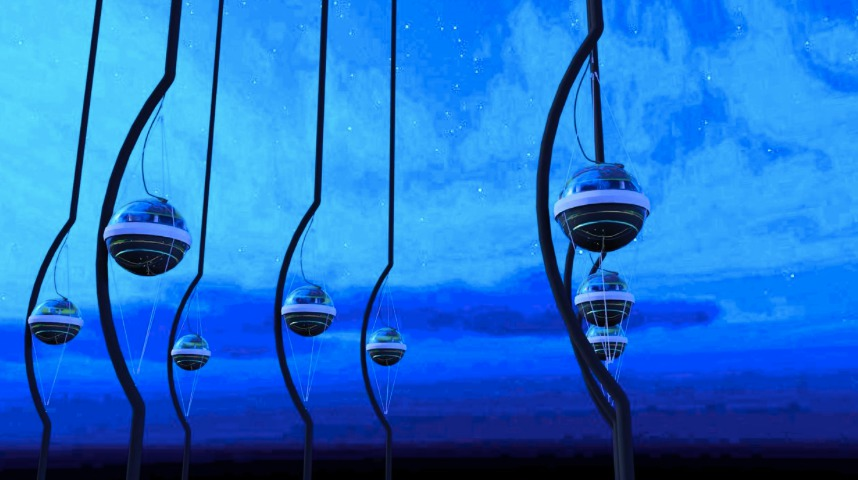
\includegraphics[width=0.5\textwidth]{Fig-01-22.jpg}
\end{figure}